\documentclass{article}
\usepackage{graphicx} % Required for inserting images
\usepackage[utf8]{inputenc}

\title{SemRestore-QA: Abstract for Soch Vichar Achar 2026}
\author{ResCon, IIT Bombay}
\date{October 2026}

\begin{document}

\begin{center}
\textbf{\Large SemRestore-QA: Do Image-Quality Metrics Notice When Restoration Changes the Content?} \\[2em]
\textbf{Abhishek Singh (EECS), Piyush Pritam (DSE), Mrinal Negi (EECS)} \\[0.5em]
\textbf{Supervisor: Samiran Das (DSE)} \\[0.8em]
\textit{Departments of Electrical Engineering and Computer Science (EECS) and}\\
\textit{Data Science and Engineering (DSE), IISER Bhopal}
\end{center}

\vspace{2em}

\section*{Abstract}

\begin{itemize}

\item \textbf{\textit{Purpose}}: Generative restorers (GANs, diffusion), now used in phone cameras, forensics, driving and medical imaging, can output sharp images with wrong content. HalluGen [1] showed on brain MRI that PSNR, SSIM and LPIPS can rank such hallucinations above slightly blurred but correct outputs. We contribute (1) a natural-image benchmark of four content changes with PSNR-matched faithful controls and (2) SemRestore, a localized metric that catches all four.

\item \textbf{\textit{Method}}: From 120 COCO images [3] (60 tuning, 60 held out) we made 403 edits with known masks: addition and substitution (Stable Diffusion inpainting), removal (LaMa) and recolor (hue shift, three severities), filtered by CLIP. Each edit got blurred and noised copies of the clean photo at equal PSNR (within 0.1~dB). SemRestore extends SHAFE [1]: DINOv2 [2] patch distances plus a colour map, calibrated against blur and noise, then pooled into a score and a heatmap. It was frozen on the tuning split before one held-out test run (bootstrap 95\% CIs); our SHAFE matches the official code exactly. Edited images were also super-resolved by regression, GAN and diffusion models.

\item \textbf{\textit{Results}}: At equal PSNR, LPIPS preferred the edit in 98\% of blur pairs; SSIM and DISTS were also below chance (Fig.~1). SHAFE-DINO caught object edits (AUROC 0.98--1.00) but not recolouring (0.54), as DINOv2 largely ignores colour. SemRestore reached AUROC 0.95--0.97 on all four types and preferred the faithful image in 98\% [95--99] of blur pairs and 100\% of noise pairs; at 5\% false alarms it missed 24\% of edits (SHAFE-DINO: 54\%). Its heatmap hit the edit every time, and AUROC stayed 1.00 on restored edits for all three families.

\item \textbf{\textit{Conclusions}}: Common metrics reward sharp but wrong restorations on natural photos too. A calibrated colour channel added to localized feature comparison closes this gap, though severity ranking stays weaker than with pixel metrics. A blinded human study is ongoing.

\end{itemize}

\begin{figure}[h]
\centering
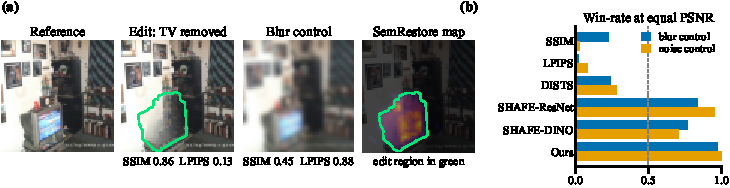
\includegraphics[width=\linewidth]{figure1.pdf}
\caption{(a) Held-out example at equal PSNR: SSIM and LPIPS prefer the edit; our map marks the change. (b) Faithful-image win-rate (0.5 = chance).}
\end{figure}

\section*{Acknowledgements}
Course project for DSE312 Computer Vision, IISER Bhopal.

\section*{References}

\begin{enumerate}
\item S.~Kim \textit{et al.}, ``HalluGen: Synthesizing Realistic and Controllable Hallucinations for Evaluating Image Restoration,'' CVPR 2026.
\item M.~Oquab \textit{et al.}, ``DINOv2: Learning Robust Visual Features without Supervision,'' TMLR 2024.
\item T.-Y.~Lin \textit{et al.}, ``Microsoft COCO: Common Objects in Context,'' ECCV 2014.
\end{enumerate}

\end{document}
